% ============================================================================
\section{Methodology}
\label{sec:method}
% ============================================================================
To support the changing hardware requirements of \cref{sec:setting}, we studied four complementary axes: data and features (\cref{sec:features}), classifier and loss (\cref{sec:loss}), architecture (\cref{sec:arch}) and the input unit (\cref{sec:input_unit}). Matched comparisons isolate individual mechanisms where possible. Models are named by their inputs, architecture and training objective; \cref{tab:naming} (\cref{app:naming}) explains every name.

% ----------------------------------------------------------------------------
\subsection{Data exploration and feature engineering}
\label{sec:features}
% ----------------------------------------------------------------------------
We compared class-normalised distributions of $\tau$ and non-$\tau$ objects on the training split, overall and within the $\ptTOB$ intervals $[5,10)$, $[10,20)$, $[20,40)$, $[40,80)$ and $[80,120)\GeV$. A variable carries information beyond energy only if the classes still differ \emph{inside} each interval. All features live in a modular registry and are selected by configuration (\cref{app:features}).

\paragraph{Energy: a strong separator and a shortcut.}
$\ptTOB$ is the strongest single separator (\cref{fig:features}a). Non-$\tau$ objects pile up at the $\SI{5}{GeV}$ threshold, while $\tau$ objects have a long tail. For the same reason it is a \emph{shortcut}: a network trained with BCE lowers its loss by learning the energy scale and has little incentive to learn the weaker, complementary shape information. This observation motivated the classifier of \cref{sec:loss}.

\paragraph{EM2 compactness.}
The most useful engineered variable is the fraction of the $12\times12$ EM2 energy contained in its most energetic $3\times3$ cell window:
\begin{equation}
  \Frac=\max_{w\in\mathcal{W}}\sum_{(a,b)\in w}E_{ab}\Big/\sum_{a,b}E_{ab},
  \label{eq:frac}
\end{equation}
where $\mathcal{W}$ is the set of the $100$ overlapping $3\times3$ windows (\cref{fig:features}c,d). A cell window is smaller than one tower, so $\Frac$ measures compactness at a granularity the core tensor cannot resolve. Unlike $\ptTOB$, its separation persists within fixed energy intervals and grows with energy (\cref{fig:features}b, \cref{fig:frac_conditioned}).

\begin{figure}[t]
  \centering
  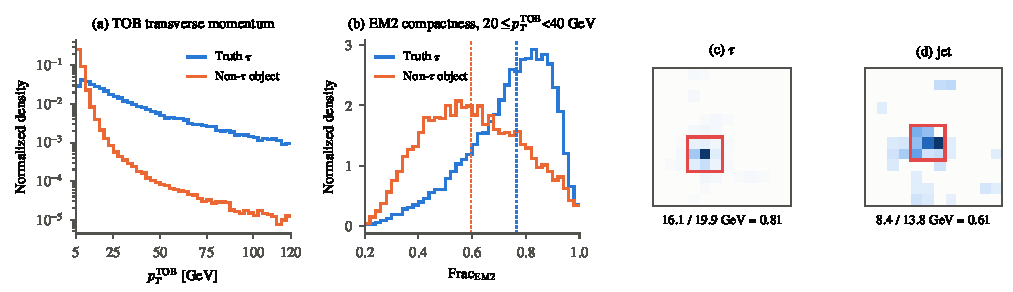
\includegraphics[width=0.95\linewidth]{figures/fig_features.pdf}
  \caption{Feature study (training split, normalised per class). (a) $\ptTOB$, log scale. (b) $\Frac$ for $20\leq\ptTOB<\SI{40}{GeV}$; dashed lines mark the medians. (c,d) Computation of $\Frac$ for the objects of \cref{fig:calo_input}: the red square is the best $3\times3$ window.}
  \label{fig:features}
\end{figure}

\paragraph{Inputs used below.}
Besides $\Frac$ (\Ffeat), four inputs stayed competitive at the operating point:
the 45 raw core cells (\CT), the strongest single input throughout;
15 per-layer summaries (\SUM), which are the sum $S_\ell$, the dominance $2M_\ell-S_\ell$ ($M_\ell$ the maximum cell) and the sparsity $\#\{\text{cells}>0.1M_\ell\}$ of each layer~\cite{kernan2026};
the ``core physics'' vector (\CP): BDT score, $\ptTOB$, and $\eta,\phi$ relative to the leading TOB;
and the EM2 image, which only the CNNs read.
Event-topology variables (the $\ptTOB$ sum, the second-highest $\ptTOB$, the separation of the two leading TOBs) clearly separate events by $\tau$ multiplicity. However, they take the same value for every object of an event, cannot rank the objects within it, and did not improve on object-level inputs at $\FPRtarget$ (\cref{sec:input_unit}, \cref{app:features}).

% ----------------------------------------------------------------------------
\subsection{Classifier and loss design}
\label{sec:loss}
% ----------------------------------------------------------------------------
BCE measures the average quality of object-level probabilities. The trigger instead depends on the far tail of the \emph{event-level} background distribution and has explicit requirements per energy region. We addressed this mismatch in three steps, each changing one mechanism: the decision rule, the signal weighting and the training objective.

\paragraph{The TOB--NN OR classifier.}
Instead of asking a network to relearn the energy threshold, we pair it with the deterministic TOB comparator: accept an object through either branch, then require two accepted objects per event,
\begin{equation}
  a_{e,i}=\1[\ptTOBof{e,i}\geq C]\vee\1[s_{e,i}\geq t],\qquad A_e=\1\Big[\textstyle\sum_i a_{e,i}\geq2\Big].
  \label{eq:or}
\end{equation}
The TOB branch protects the high-energy plateau; the NN supplies complementary shape-based decisions. Thresholds are calibrated jointly, counting mixed-branch events exactly. Validation selects the TOB budget $b$ to maximise the equally weighted efficiency gain across $25$--$100\GeV$, subject to the event fake-rate limit and regional protection guards. A smaller selected $b^\star$ suggests less reliance on the comparator, not a standalone measure of NN quality. Training remains (weighted) BCE; the OR changes the decision rule only. \Cref{app:or} gives the objective, cross-fitted calibration, guards and earlier two-expert trial.

\paragraph{Spectrum-aware signal weighting.}
We reweight each object's contribution to binary cross-entropy:
\begin{equation}
  \mathcal L_{\mathrm{wBCE}}=-\frac1N\sum_i w_i\big[y_i\log s_i+(1-y_i)\log(1-s_i)\big],
  \label{eq:weighted_bce}
\end{equation}
where $y_i$ is the signal label and $s_i$ the NN score. Background keeps $w_i=1$; for signal, $w_i=r(t_i)/\langle r\rangle_{\mathrm{train},S}$, with truth momentum $t_i$ in GeV. Mean-one normalisation preserves the total signal weight while redistributing its gradient across energies. We compare two raw profiles:
\begin{equation}
  \begin{aligned}
    r_{\mathrm{IF}}(t)&=\operatorname{clip}\!\left(\bar n/n_{k(t)},\,0.2,\,5\right),
    & r_p(t)&=\operatorname{clip}(t,10,200)^{-p}.
  \end{aligned}
  \label{eq:powerlaw}
\end{equation}
\emph{Inverse frequency} (IF) uses the training-signal count $n_k$ in each populated $5\GeV$ bin over $25$--$100\GeV$, with $\bar n$ their mean; outside these bins, $r_{\mathrm{IF}}=1$. Rare bins receive larger weights, approximately balancing their total influence. \emph{Power-law weighting} varies smoothly: $p=-1$ doubles the weight when energy doubles away from the clamp, whereas $p=0$ recovers BCE. Since soft taus dominate the sample, both IF and negative $p$ shift learning towards rarer, cleaner energetic examples without resampling the data. This often helped more than further emphasising ambiguous low-energy taus, but depended on the inputs. Full profiles, scans and the transfer hypothesis appear in \cref{app:weighting}; comparisons are in \cref{app:analysis_weighting}.

\paragraph{A constrained trigger objective.}
A fixed weight profile applies the same emphasis whether or not a protection is at risk. Our last step therefore optimises the trigger objective itself. It had a second, more general aim: to find out what a loss that truly represents the trigger problem must look like, and which properties it must have. We collect these conclusions in \cref{sec:lessons}. The problem is
\begin{equation}
  \max_\theta\sum_{k\in\Kset_J}w_k\big[\eff_k(\theta)-\effTOB_k\big]\quad\text{s.t.}\quad\FPRev(\theta)\leq\FPRtarget,\;\;\eff_k(\theta)\geq r_k\;\;(k\in\Kset_C).
  \label{eq:constrained}
\end{equation}
The Lagrangian rewards turn-on gains while penalising fake-rate and regional
deficits. Training uses smooth decisions; exact out-of-sample checks,
threshold recalibration, temperature annealing and uncertainty-aware
fine-tuning stabilise the optimisation (\cref{app:constrained}).

% ----------------------------------------------------------------------------
\subsection{Architectures}
\label{sec:arch}
% ----------------------------------------------------------------------------
Every model in this paper is assembled from the same parts (\cref{fig:arch}a). Optional convolutional branches read the core tensor and the EM2 image, their outputs are concatenated with scalar inputs, and a $[32,16]$ dense head produces the object score. The model names in \cref{tab:naming} describe which parts are used.

\paragraph{MLP.}
The reference model is the $[32,16]$ ReLU MLP with a sigmoid output of~\cite{kernan2026}. On the 45 core cells plus $\Frac$ (\CT+\Ffeat, 46 inputs) it has $2{,}049$ parameters. Larger MLPs did not help~\cite{kernan2026}, so we looked for a better inductive bias rather than more capacity.

\paragraph{Convolutions on the core tensor.}
A flat MLP must learn from data that neighbouring cells are adjacent. A convolution builds in locality and weight sharing instead. Many hand-made features are in fact fixed convolutions followed by pooling; $\Frac$, for example, is an all-ones $3\times3$ kernel, a global maximum and a division. We tested four backbones on the $5\times3\times3$ tensor. V1 mixes the five layers at every cell ($1\times1\times5$ kernel) and learns longitudinal profiles. V2 learns local spatial patterns ($2\times2\times5$ kernel). V3 applies them in series, and V4 in parallel. Because the window is centred on the TOB seed, position matters, so the maps are flattened rather than pooled. \Cref{app:vbackbones} explains each backbone step by step, and \cref{fig:cnn_blocks}a draws them.

\paragraph{A branch for the full-granularity EM2 layer.}
Following~\cite{ayyar2020cnn,icecube2025cnn,kim2023hotspots}, the $12\times12$ EM2 image gets its own branch. E1 applies one $3\times3$ convolution with four filters and $2\times2$ max pooling. E2 adds a second convolution block. E3 learns its down-sampling with a stride-2 convolution. The \emph{dual-branch} model concatenates a V-backbone, an E-branch and optionally $\Frac$ into one head. \Cref{app:ebranches} and \cref{fig:cnn_blocks}b give the details.

\paragraph{Is $\Frac$ still needed next to the EM2 branch?}
Although $\Frac$ is derived from EM2, a small CNN need not learn its global normalisation easily. We therefore compare matched models with and without the scalar: does an explicit scale-free ratio complement learned local patterns? The ablation is reported in \cref{app:analysis_representation}; the architectural rationale is in \cref{app:fraction_complementarity}.

\paragraph{Towards a smaller model: EM2 only.}
EM2's strong contribution motivated removing the core convolution, but not the core measurements: the 45 cells or 15 layer summaries enter the dense head as scalars beside the E-branch and $\Frac$. This tests whether spatial processing is worth its parameter cost (\cref{app:em2only,app:analysis_representation}).

\paragraph{Stability and simplicity.}
Every convolution is followed by BatchNorm~\cite{ioffe2015batchnorm} and LeakyReLU~\cite{maas2013leaky}, which keeps training stable on this highly imbalanced data. Inputs are standardised energies (\cref{app:arch}). Their performance is compared in \cref{sec:analysis}. All parameter counts are listed in \cref{tab:params}.

\begin{figure}[t]
  \centering
  \resizebox{0.95\linewidth}{!}{% Architecture and event-decision diagram (TikZ). Included from Sec. 4.3.
\definecolor{archblue}{HTML}{2A78D6}
\definecolor{archorange}{HTML}{EB6834}
\definecolor{archink}{HTML}{52514E}
\begin{tikzpicture}[
  font=\scriptsize,
  >={Stealth[length=1.4mm]},
  box/.style={draw=archink, rounded corners=1.5pt, align=center, inner sep=1.8pt, line width=0.4pt, minimum height=6.5mm},
  inp/.style={box, fill=archblue!7, text width=15mm},
  conv/.style={box, fill=archblue!22, text width=20mm},
  dense/.style={box, fill=archink!10},
  acc/.style={box, fill=archorange!14, text width=23mm, minimum height=5mm},
  obj/.style={box, fill=archblue!7, minimum width=6mm, minimum height=5mm},
  arr/.style={->, draw=archink, line width=0.45pt},
  lbl/.style={font=\footnotesize\bfseries},
  note/.style={font=\tiny, text=archink, align=center}
]
% ---------------- (a) single-object model ----------------
\node[lbl] at (-0.55,1.25) {(a)};
\node[inp]  (ct)   at (0.25, 0.75) {core tensor\\$5\times3\times3$};
\node[inp]  (em2)  at (0.25,-0.15) {EM2 image\\$12\times12$};
\node[inp, minimum height=5mm]  (frac) at (0.25,-0.95) {$\Frac$};
\node[conv] (ctb)  at (2.45, 0.75) {backbone V1--V4\\(layer mix / spatial)};
\node[conv] (emb)  at (2.45,-0.15) {branch E1--E3\\(conv, pool / stride)};
\node[circle, draw=archink, inner sep=0.5pt, line width=0.4pt] (cat) at (4.05,0.30) {$\oplus$};
\node[dense, text width=14mm] (head) at (5.05,0.30) {dense $[32,16]$\\+ sigmoid};
\node (s) at (6.3,0.30) {$s_{e,i}$};
\draw[arr] (ct) -- (ctb);
\draw[arr] (em2) -- (emb);
\draw[arr] (ctb.east) -- (cat);
\draw[arr] (emb.east) -- (cat);
\draw[arr] (frac.east) -| (cat.south);
\draw[arr] (cat) -- (head);
\draw[arr] (head) -- (s);
\node[note] at (2.45,1.30) {conv\,$\to$\,BatchNorm\,$\to$\,LeakyReLU};
% ---------------- (b) event decision ----------------
\begin{scope}[xshift=7.25cm]
\node[lbl] at (-0.35,1.25) {(b)};
\foreach \k/\y in {1/0.88,2/0.25,3/-0.38} {
  \node[obj] (x\k) at (0.1,\y) {$x_{e,\k}$};
  \node[dense, minimum height=5mm] (f\k) at (0.95,\y) {$f_\theta$};
  \node[acc] (a\k) at (2.7,\y) {$s_{e,\k}\!\ge\! t\;\vee\;q_{e,\k}\!\ge\! C$};
  \draw[arr] (x\k) -- (f\k);
  \draw[arr] (f\k) -- (a\k);
}
\node at (0.1,-0.78) {$\vdots$};
\node at (0.95,-0.78) {$\vdots$};
\node at (2.7,-0.78) {$\vdots$};
\node[note] at (0.5,-1.15) {shared weights, $\leq6$ TOBs};
\node[box, fill=archblue!22, minimum height=6mm] (cnt) at (4.95,0.25) {$\sum_i a_{e,i}\geq2$};
\node (Ae) at (6.2,0.25) {$A_e$};
\foreach \k in {1,2,3} { \draw[arr] (a\k.east) -- (cnt.west); }
\draw[arr] (cnt) -- (Ae);
\node[note] at (4.95,-0.42) {calibrated to\\$\FPRev\leq0.5\%$};
\end{scope}
\end{tikzpicture}
}
  \caption{Overview of the single-object pipeline. (a) How every model is assembled: optional convolutional branches on the core tensor (V1--V4) and on the EM2 image (E1--E3), concatenated with scalar inputs such as $\Frac$, feed a $[32,16]$ head. The MLP uses flat inputs only. (b) How object scores become an event decision (\cref{sec:setting,sec:input_unit}): one shared network scores every TOB; the OR classifier also accepts an object when $q_{e,i}=\ptTOB\geq C$; the event fires with at least two accepted objects.}
  \label{fig:arch}
\end{figure}

% ----------------------------------------------------------------------------
\subsection{Input unit: single-object and pair-object models}
\label{sec:input_unit}
% ----------------------------------------------------------------------------
\paragraph{Single-object models.}
All models above score each TOB independently, with one shared network applied to that object's inputs. The event decision is taken afterwards by the counting rule~\eqref{eq:event_decision} or by the OR rule~\eqref{eq:or} (\cref{fig:arch}b). The decision is therefore independent of TOB order. One small circuit can be replicated for every TOB slot. Training uses object labels, while calibration and evaluation are done at event level. The price is that the network sees no event context: an event-level input is identical for all objects of an event, so it cannot rank them.

\paragraph{Pair-object models.}
We score every unordered pair of finite-$\ptTOB$ TOBs from the same event.
Both members use the same encoder; the complete model has $4{,}357$ parameters.
Its inputs are the
fine EM2 image, coarse cells, measured $\ptTOB$, $\Frac$ and event context.
Same-label pairs teach the model; inference scores all pairs. Training averages
weighted BCE within each eligible event, then averages those event losses.
This removes extra weight from pair multiplicity; signal weights still vary.
Details and \eqref{eq:pair_event_loss} appear in \cref{app:pair_protocol}.

The neural event score is $s_e=\max_{(i,j)\in\mathcal P_e}s_{e,ij}$;
$q_e$ is the second-highest finite $\ptTOB$. The joint decision is
\begin{equation}
  A_e=\1[s_e\geq t]\vee\1[q_e\geq C].
  \label{eq:pair_decision}
\end{equation}
Both branches share one event-level background budget. Checkpoints and
thresholds are selected on validation independently for each training seed;
the models are not combined into an ensemble. Events without a pair receive
a non-passing score and remain in the evaluation denominators.
